\section{数值可信度与参数灵敏度}

本题没有药材内部温度与含水率的实测剖面，附件只给出烘房环境与外轮廓半径。
以下证据是模型的内部一致性与数学正确性，不能解释为与实测吻合；
唯一具有外部性质的比对是问题一的级数解，它属于同一模型的独立解法而非独立观测\upcite{Pelletier2000}。

\subsection{离散守恒与收敛性}

把控制体内含水量的累积变化与表面净流出相比，相对残差为

\begin{equation}\label{eq:resid}
\varepsilon=\frac{\left|\displaystyle\sum_i V_i\bigl[C_i(t)-C_i(0)\bigr]
+\int_0^{t}2\pi R\,h_m\bigl[C(R,\tau)-C_{\rm air}(\tau)\bigr]\mathrm{d}\tau\right|}
{\displaystyle\sum_i V_i\,C_i(0)} .
\end{equation}

式~\eqref{eq:resid} 检验的是离散方程中储存项与控制体通量的数值平衡，
而非真实系统总水分质量守恒误差。问题一、问题三与问题四的残差分别为
$7.41\times10^{-16}$、$1.55\times10^{-14}$ 与 $7.51\times10^{-16}$，均已接近双精度机器精度。
正式配置见公共模型末段。达标时长对网格与步长的敏感性见图~\ref{fig:convergence}。

\begin{figure}[H]
  \centering
  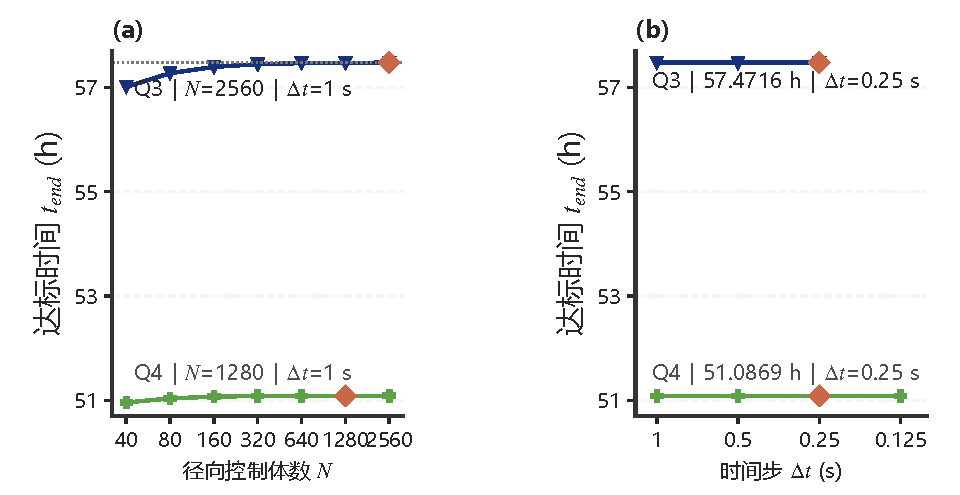
\includegraphics[width=0.76\textwidth,height=0.30\textheight,keepaspectratio]{../figures/fig_convergence.pdf}
  \caption{问题三与问题四的空间和时间步收敛性}
  \label{fig:convergence}
\end{figure}

面板 (a) 为问题三与问题四在 $\Delta t=1$~s 下由 $N=40$ 至 $N=2560$ 的空间收敛；
面板 (b) 为各自正式配置下的时间步收敛。对应达标时长分别为 $57.4716$~h 与 $51.0869$~h。

\subsection{物理合理性与极限退化}

四问结果一致满足：含水率对时间单调不增；同一时刻中心含水率不低于表面、中心温度不高于表面；
全场有界且无负值，正式结果含水率不低于 $0.0526$，$4$~h 后环境稳态外推为 $50.0000~^\circ$C 与 $0.0500$~kg/kg。
问题一的「热先于质」亦得到确认。中心温度在环境小幅回落时出现 $5.2\times10^{-5}~^\circ$C 的极小回落，
幅度小于同期环境回落 $7.5\times10^{-3}~^\circ$C 的百分之一，属边界扰动向内衰减，而非时间推进振荡。

移动边界还须在退化情形回到固定域。令 $\dot R\equiv0$，
式~\eqref{eq:landau_T}--\eqref{eq:landau_C} 的表观对流恒为零，
$\chi=1$ 与 $\chi=0$ 给出相同达标时长。另令 $h_m$ 取很大值，$1$~h 时表面含水率与 $C_{\rm air}$ 之差为 $1.7\times10^{-15}$，
说明式~\eqref{eq:bc_surface} 的方向与符号正确。

\subsection{参数灵敏度}\label{sec:sens}

参数分三类：题给确定量、经验公式中带拟合不确定性的量，以及建模选择引入的量。
对第二、三类作一次一因子扰动，达标时长响应见图~\ref{fig:q3_sensitivity}。

\begin{figure}[H]
  \centering
  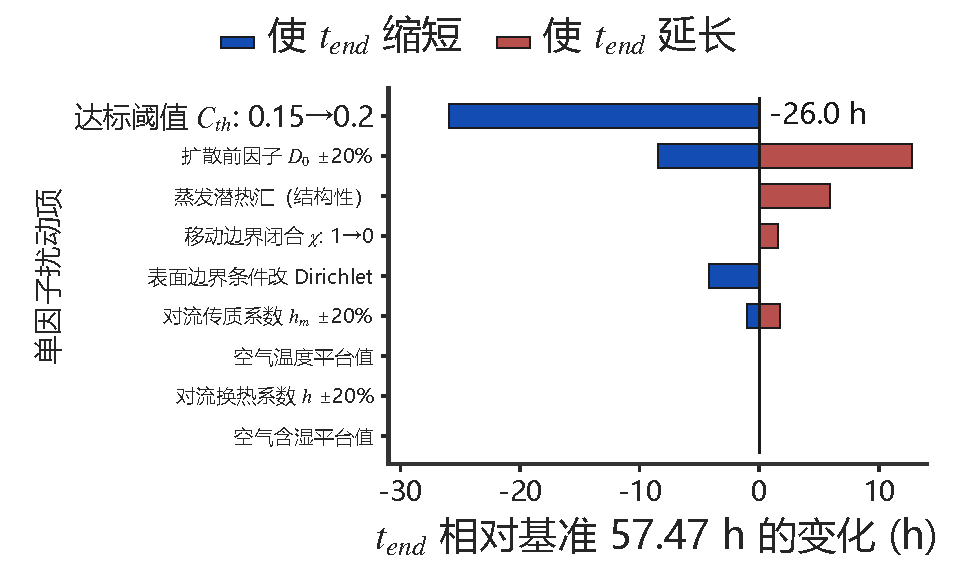
\includegraphics[width=0.70\textwidth,height=0.26\textheight,keepaspectratio]{../figures/fig_q3_sensitivity.pdf}
  \caption{达标时长的最终精度单因子灵敏度诊断}
  \label{fig:q3_sensitivity}
\end{figure}

最终精度诊断中，扩散系数前因子 $\pm20\%$ 带来 $-8.43$ 至 $+12.76$~h 的变化，
弹性约 $-0.73$ 至 $-1.11$，是最强不确定度来源；对流传质系数同幅扰动为
$-1.04$ 至 $+1.70$~h，弹性约 $-0.09$ 至 $-0.15$；对流换热系数仅 $0.02$~h 量级，
弹性约 $-0.001$ 至 $-0.002$。排序印证本题由内部扩散控制，表面换热几乎不影响时长，
精度关键在扩散系数经验式而非对流系数。以附件 1 末 $30$ 个样本均值 $50.0105~^\circ$C 和 $0.049982$~kg/kg
替代外推值后，时长变化均低于 $0.04\%$，说明结果对该外推不敏感。

达标阈值是工艺规定而非模型参数。基于 \verb|result3.xlsx| 的 $60$~s 正式输出作线性插值后处理，
阈值由 $0.15$ 改到 $0.20$~kg/kg 会使时长缩短 $25.96$~h，即近一半。
工艺上把安全水分放宽 $0.05$~kg/kg，时间收益远大于模型改进——前提是贮藏安全性允许。

结构性选择一并探查。改用第一类边界会缩短时长。取汽化潜热近似 $\lambda=2.4\times10^6$~J/kg，
计入潜热后问题三时长由 $57.4716$~h 增至 $63.4189$~h，增幅约 $10.35\%$，
说明忽略潜热会使预测偏短。该计算只评估方向与量级，不作为正式结果的精确修正。
两项探查都不改变交付结果：题面已给出对流系数（即第三类边界），也未给出潜热数据。
